\chapter{Testing and Results}
The delivered improved version of Issie was tested from three perspectives. These were \textbf{correctness}, \textbf{performance}, and \textbf{user experience}. Testing the correctness of the improvements made to Issie included checking that the implemented functionality worked as intended, as well as ensuring that the application was stable, not crashing regardless of user input. Quantitative performance testing was conducted by first measuring the average time taken for specific actions and processes, and then those measurements to Robert Miller's \cite{Miller1968ResponseTI} classes for perceived responsiveness of an application. Finally, the quality of the user experience was evaluated by giving survey participants a series of tasks in Issie, measuring their performance, and collecting their feedback.

\section{Testing Application Stability} \label{sec:testappstability}
An application is considered stable when the user is not subjected to undefined behaviour or inexplicable crashes while using the application. The stability of the improved version of Issie delivered by the project was verified by analysing cases in the codebase which could trigger a system crash, and systematically evaluating that they could not occur. There are two scenarios which can cause Issie to crash:
\begin{itemize}
    \item Un-handled exceptions: exceptions can either be generated by the developer or can be generated by library functions. If these exceptions are not caught and handled appropriately, the cause the application to crash.
    \item When \codestyle{failwithf} is called in the code: this function is called when an unexpected case that should never occur is matched in the code. An example of this would be if the Update function receives the instruction to reduce a truth table with Don't Cares when no truth table exists.
\end{itemize}

\subsection{Exception Analysis}
The code added to Issie was analysed to explore the scenarios in which exceptions could be raised. Exceptions are uncommon in F\fsharp -- instead the use of Monad types such as \codestyle{Option} and \codestyle{Result} is preferred. When using Monad types, failure of an operation is an option and the programmer is made to account for the possibility of it while programming. In contrast, functions which return exceptions place the onus of verifying the arguments prior to the call on the developer. An example of this is the difference between the functions \codestyle{Map.find} and \codestyle{Map.tryFind}; both functions look up a key in a Map and return the corresponding value, but return the value in different ways. When a key exists, \codestyle{Map.find} returns the value, but when it does not exist it raises an exception. If the developer fails to account for this, the program may crash unexpectedly. In contrast \codestyle{Map.tryFind} wraps the returned value in the \codestyle{Option} type, and returns \codestyle{Some value} if the key exists in the Map, or \codestyle{None}. Therefore, when using \codestyle{Map.tryFind}, the developer must always actively handle the failure case at that point in the code, either providing alternate behaviour or manually making the choice to fail the application with \codestyle{failwithf}. This significantly reduces the chance of application crashes due to an oversight made by the developer with regard to exception handling. 

All library functions used in the code written during the project were analysed, and it was checked which of the ones used could possibly return any exceptions. For each of these functions a strategy was devised to check whether an exception could occur in practice:

\begin{table}[ht]
    \centering
    \begin{tabular}{|m{3cm}|m{9cm}|m{2cm}|}
    \hline
        Function &  Check & Pass/Fail\\ \hline
        \codestyle{List.except} & Ensure that the items to exclude sequence can never be null. & Pass \\\hline
        
        \codestyle{List.head} & Ensure that the supplied list is not empty either through a conditional statement or pattern match case on the list. & Pass \\ \hline
        
        \codestyle{List.updateAt} & Ensure that the index is valid (between 0 and length-1) either through a bounds check or from properties. & Pass \\ \hline
        
        \codestyle{Seq.allPairs} & Ensure that the both sequences can never be null. & Pass \\\hline
        
        \codestyle{Seq.append} & Ensure that the both sequences can never be null. & Pass \\\hline
        
        \codestyle{Seq.init} & Ensure that the count can never be negative. & Pass \\\hline
        
    \end{tabular}
    \caption{Library functions in project code which can throw exceptions}
    \label{tab:exceptions}
\end{table}

Exceptions can also be raised in the code by the developer if required, and caught using a \codestyle{try-catch} block. This project only adds one such exception; the \codestyle{AlgebraNotImplemented} exception which is be raised in the Fast Simulation function \codestyle{fastReduce} when algebra is passed to an unsupported port or component. An exception is used here because manually propogating a \codestyle{SimulationError} up the call stack would be very impractical. The \codestyle{AlgebraNotImplemented} exception contains a \codestyle{SimulationError} data structure; whenever there is a scenario in which algebra is fed to the Fast Simulation, there is a \codestyle{catch} block waiting to catch any the exception and return the \codestyle{SimulationError} contained within. Additionally, the XML documentation of functions in the Fast Simulator has been updated to reflect the new exception. Therefore, it can be said that the code added by this project to Issie is stable from an exception point-of-view.

\subsection{Failure Analysis}
To ensure that the application could not fail during use, every \codestyle{failwithf} case in the project code was inspected, and a summary made of the scenarios in which the function would be called. Once the scenario was ascertained, one of two actions woere taken. If the fail case was related to application state, it was ensured through thorough inspection of the code that such a state could never occur. If the fail case was related to the UI, testing involved attempting to create those circumstances in the application. In all cases, attempts to achieve scenarios that would call the application to fail and exit were unsuccessful. 

In addition to exception and failure analysis, the completed application has been used for other purposes for long periods of time. The process of repeatedly testing the correctness of other features totalled over 3 hours, in which multiple tasks were carried out using the application. Additionally, during user experience testing, not a single user reported any crashes or undefined behaviour. This supports the notion that the code added to the project is robust and stable, and that all situations with erroneous user input have been handled.

\section{Correctness Testing}
Correctness of the implemented features was tested by testing the features on 6 different circuits, each of varying complexity. These circuits can be described as:
\begin{itemize}
    \item A two-input multiplexer circuit implemented only using gates
    \item A circuit containing a Mux4 component with 2-bit inputs to each data line of the multiplexer
    \item A circuit which calculates the bitwise And of two 8-bit inputs
    \item A Full Adder circuit using a Half Adder custom component, all built exclusively from logic gates
    \item A circuit which either adds or subtracts two 16-bit values depending on the selected mode
    \item An 8-bit ALU, which is a custom component in the design of an 8-bit CPU
    \item An 8-bit CPU design
\end{itemize}

A summary of the tested features can be found in Table \ref{tab:test}. All of the tested features worked as intended for all schematics, indicating that they have been implemented correctly and will therefore work reliably when distributed to real-world users.

\begin{longtblr}[
  caption = {List of all features which were manually tested},
  label = {tab:test},
]{
  colspec = {|X[5]|X|},
  rowhead = 1,
  hlines,
} 
\textbf{Feature Checked} & \textbf{Pass/Fail} \\
For all combinational circuits, a numeric truth table can be generated for the whole sheet.  & Pass \\
For all valid selections of a schematic, a numeric truth table can be generated:
\begin{enumerate}
        \item The selected canvas is corrected successfully, with newly generated input or output components.
        \item Newly generated IOs are labelled based on which component ports they connect to.
        \item Truth tables for selections can be generated even if errors or sequential components exist elsewhere in the schematic.
    \end{enumerate} & Pass \\
If there are errors in the schematic, the \textit{See Problems} button appears in place of the \textit{Generate Truth Table} button, and clicking it conveys the error to the user.  & Pass \\
Users are prevented from generating truth tables for schematics containing sequential logic, and this reason is conveyed to them. & Pass \\
For all circuits where the total width of all the inputs combined exceeds 10 bits, a truncated truth table of 1024 rows is displayed, along with a warning notification informing the user about the truncation.  & Pass \\
The base of numbers in the truth table can be changed using the base selector.  & Pass \\
Truth table related functionality can be shown and hidden by expanding and closing menu sections.  & Pass \\
Input constraints can be applied to the truth table and successfully change the input state so that rows that were previously truncated are now generated and displayed.  & Pass \\
Significantly restrictive input constraints will reduce the input space enough so the truth table will no longer be truncated.  & Pass \\
Output constraints filter the existing truth table.  & Pass \\
There is an intuitive interface for adding/removing constraints:
\begin{enumerate}
    \item Clicking on the \textit{Add} button opens the constraint editor popup.
    \item Changing the chosen IO in the IO selection section updates the IO displayed in the editor section.
    \item Real-time validation of constraints is performed as they are entered, with errors clearly conveyed to the user.
    \item Constraints that are currently being applied are clearly displayed to the user with tags, and can be deleted easily by clicking the cross next to them.
    \item All constraints can be cleared in one go with the \textit{Clear All} button.
\end{enumerate} & Pass \\
Columns in the truth table can be hidden by using the column hider toggles.  & Pass \\
Rows in the truth table can be sorted based on a chosen IO, in ascending and descending order.  & Pass \\
The sorting information is conveyed to the user successfully through the highlighting of the relevant sorting arrow.  & Pass \\
The order of columns in the truth table can be changed.  & Pass \\
Non-truncated truth tables can be reduced with Don't Cares, with the resultant table containing no redundant rows.  & Pass \\
Users are prevented from DC reducing truncated truth tables.  & Pass \\
Users can change some or all inputs to algebra in the truth table:  
\begin{enumerate}
    \item Clicking the algebra button always spawns the algebra selector popup, where inputs can be toggled between numeric and algebraic values.
    \item If a certain input is not supported as being algebraic, the user is informed of the reason why. They are prevented from applying the incompatible algebraic inputs.
    \item When algebraic inputs are in the truth table, the outputs are informative algebraic expressions which is a correct function of the inputs.
\end{enumerate} & Pass \\
Algebraic reduction rules are applied correctly, yielding correctly simplified algebraic expressions at the outputs  & Pass \\
Algebraic expressions are printed correctly in the truth table.  & Pass \\
When the truth table tab is open, width of the right section can be changed using the draggable dividerbar.  & Pass \\
The truth table is responsive:
\begin{enumerate}
    \item Changing the width of the right section changes the width of the truth table (therefore of the columns in the table).
    \item When the content inside a truth table cell is too wide, the height of the row automatically adjusts so that the content can wrap to the next line.
    \item Operations on the truth table appear instantaneous.
\end{enumerate} & Pass \\
The waveform simulation can successfully be run from the new Waveform Simulator sub-tab.  & Pass \\
\end{longtblr}

\section{Quantitative Performance Testing} \label{sec:performance}
The three following schematics were used for measuring the performance of the application, with each having slightly different attributes. All tests were performed on a MacBook Air, featuring an M1 CPU with 8GB of RAM.
\begin{enumerate}
    \item A circuit containing a Mux4 component with 2-bit inputs to each data line of the multiplexer. In total, this circuit has 5 2-bit inputs, meaning that it will generate exactly 1024 rows (no truncation required). This is a simple circuit with only one component, so should be quick to simulate. However, there are many redundancies in the truth table, so Don't Care reduction may take longer.
    \item A circuit which either adds or subtracts two 16-bit values depending on the selected mode. This circuit features slightly more complex logic than the previous one, and also will result in the truth table being truncated. This will be referred to as the 'Add Or Sub' schematic.
    \item An 8-bit ALU, which is a very complex schematic featuring lots of library and custom components. This should test the generation algorithm to the maximum.
\end{enumerate}

\subsection{Generating Numeric Truth Tables}
The time taken to generate a numeric truth table was measured for all three aforementioned schematics.
\begin{table}[!ht]
    \centering
    \begin{tabular}{|l|l|l|l|l|l|l|}
    \hline
        Sheet & Trial 1 & Trial 2 & Trial 3 & Trial 4 & Trial 5 & Average \\ \hline
        Mux4 & 52 & 58 & 51 & 49 & 51 & 52.2 \\ \hline
        Add Or Sub & 75 & 72 & 69 & 81 & 78 & 75 \\ \hline
        ALU & 697 & 702 & 700 & 697 & 702 & 699.6 \\ \hline
    \end{tabular}
    \caption{Time taken to generate a numeric truth table (ms)}
    \label{tab:timeTT}
\end{table}

\subsection{Algebraic Truth Tables}
The time taken to calculate an algebraic truth table for the 8-bit ALU was measured. The circuit had five inputs in total: A and B which were 8 bits, X and F which were 3 bits, and Cin which was 1 bit. A, B, and Cin were set as algebraic inputs for the experiment. Five trials were carried out, and the average time was calculated. 

\begin{table}[!ht]
    \centering
    \begin{tabular}{|l|l|l|l|l|l|}
    \hline
        Trial 1 & Trial 2 & Trial 3 & Trial 4 & Trial 5 & Average \\ \hline
        45 & 42 & 44 & 47 & 45 & 44.6\\ \hline
    \end{tabular}
    \caption{Time taken to generate an algebraic truth table for the ALU schematic (ms)}
    \label{tab:timeAlgTT}
\end{table}

\subsection{Don't Care Reduction}
The time taken to reduce an existing truth table using Don't Cares was measured for two schematics. The Mux4 schematic was first tested, as it contains multiple redundancies and therefore requires repeated rounds of reduction. Secondly, the 'Add Or Sub' schematic was tested. As this schematic exceeds the bit limit, the input space was limited; inputs A and B were constrained to between 0 and 16. This schematic was chosen as there are no redundant rows in the truth table, as every input contributes to the output. This represents a scenario in which no DC rows are valid, and therefore the process will stop after one round of attempted reduction.

\begin{table}[!ht]
    \centering
    \begin{tabular}{|l|l|l|l|l|l|l|}
    \hline
        Sheet & Trial 1 & Trial 2 & Trial 3 & Trial 4 & Trial 5 & Average \\ \hline
        Mux4 & 2590 & 2586 & 2589 & 2616 & 2598 & 2595.8 \\ \hline
        Add Or Sub & 265 & 263 & 260 & 259 & 263 & 262 \\ \hline
    \end{tabular}
    \caption{Time taken to reduce a numeric truth table using Don't Cares (ms)}
    \label{tab:timeDCTT}
\end{table}

\subsection{Graphical Manipulation of Truth Tables}
Using the truth table generated for the ALU schematic, the time taken to perform three graphical manipulations was measured. These manipulations were: hiding an output column, sorting the truth table, and moving a column. The ALU schematic was chosen as it will generate a truncated truth table, meaning that the maximum possible 1024 rows will be rendered. It also contains 8 IOs, which is a sizeable amount.

\begin{table}[!ht]
    \centering
    \begin{tabular}{|l|l|l|l|l|l|l|}
    \hline
        Operation & Trial 1 & Trial 2 & Trial 3 & Trial 4 & Trial 5 & Average \\ \hline
        Sorting Truth Table & 35 & 33 & 36 & 41 & 39 & 36.8 \\ \hline
        Moving a Column & 21 & 25 & 22 & 23 & 27 & 23.6 \\ \hline
        Hiding a Column & 43 & 38 & 37 & 39 & 38 & 39 \\ \hline
    \end{tabular}
    \caption{Time taken to conduct different graphical manipulations on a truth table (ms)}
    \label{tab:timeTTManip}
\end{table}

\section{User Experience Testing} \label{sec:uxtest}
The success and long-term viability of any user-facing application or platform is highly dependent on the user experience it provides. For this reason, feedback must be collected from users to evaluate whether the application is achieves its purpose, and whether it if user-friendly. User feedback was collected to answer the following questions:
\begin{enumerate}
    \item Do the added features fulfil the project aim, which is to add effective novel ways of visualising combinational logic in Issie, delivering an improved education and hardware design platform?
    \item Are these features implemented in a user-friendly manner?
\end{enumerate}

The participants of the user feedback survey consisted of a group of 12 engineering students across multiple departments at Imperial College, most of whom had some beginner-level experience with combinational logic design. Participants were chosen this way so that they would not be confused by the digital electronics concepts, and would therefore be able to fully appreciate and use the added functionality. The feedback collection process consisted of two stages; in the first stage participants were provided with the updated version of Issie, then tasked with investigating five 'mystery' Issie sheets and summarising the logical function implemented by each. They were asked to use the truth table functionality while doing so, but were not pointed to where it was located in the application. The second stage consisted of a questionnaire, in which participants were given the opportunity to evaluate their experience using Issie.

\subsection{Stage 1: Mystery Sheets}
Participants were provided with five schematics labelled \textit{mystery1} to \textit{mystery5}, and were asked to describe what each sheet did. While the instructions encouraged them to "use truth tables and other features in the Truth Tables tab", they were not told where this tab was in the app's top-level UI, nor were they instructed on how to use any of the features. This was done on purpose as Issie meant to be easy to use without explicit guidance. Through this the \textit{intuitiveness} and \textit{obviousness} of the UI for truth tables was tested. The mystery sheets increased in complexity, with the initial sheets being simple to introduce the user to the application, and later sheets being more complex to push the user to explore more and use many of the added features. Table \ref{tab:mystery} provides a summary of each mystery sheet, as well as the rationale behind using it in the survey. The purpose of this exercise was to ascertain whether the added features did indeed help users gain a better understanding of combinational logic designs. Sheets Mystery 1 to Mystery 4 had a perfect record, while only one user failed to understand what Mystery 5 was doing.

\subsection{Stage 2: Questionnaire}
Once the participants had a chance to use Issie's truth table features, they were asked a series of questions about their experience. These questions fell into two categories. In the first section, they were presented with a five statements and asked to respond to them ranking them on a scale of 1 - 5, with 1 corresponding to "Strongly Disagree" and 5 corresponding to "Strongly Agree". The aim of this part of the questionnaire was to judge the quality of the user experience from different angles. The responses to this first set of questions were aggregated into a score by taking the average. Table \ref{tab:strongqs} shows the score for each statement, as well as the rationale behind why the statement was included in the questionnaire.

The second set of questions in the questionnaire focused on determining the discoverability of the implemented features. Features in an application are only useful if they are discovered by the user, so observing which features are found is important. In addition to asking whether a named feature was found, the questions also asked if they found the feature useful. The rates of discovery and usefulness -- i.e. the percentage of participants who discovered the features and found them useful, is shown in Figure \ref{fig:discgraph}.

\begin{table}[h]
    \centering
    \begin{tabular}{|m{4.2cm}|m{7cm}|m{2cm}|}
    \hline
        \textbf{Diagram} & \textbf{Explanation of Mystery Sheet} & \textbf{Score} \\
        \hline
        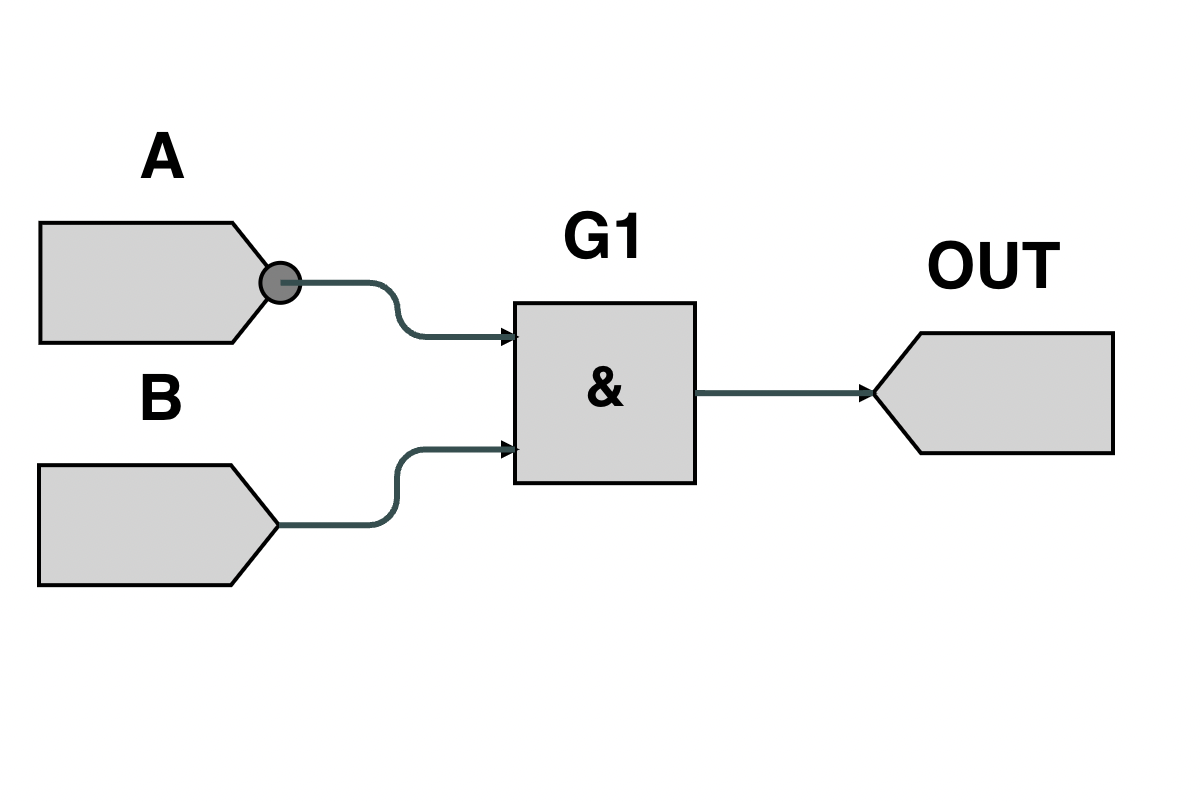
\includegraphics[width=4cm]{06.TestRes/m1.png} & \textbf{Mystery 1: Simple And Gate} The first mystery sheet was intentionally made very easy. This was done to allow users to familiarise themselves with the application and the truth table generation method. The truth table for an AND gate is very basic and is one of the first things engineering students learn. The idea was that participants would be able to use this as a reference to understand the look and feel of truth tables in Issie. & 100\% \\ \hline
        
        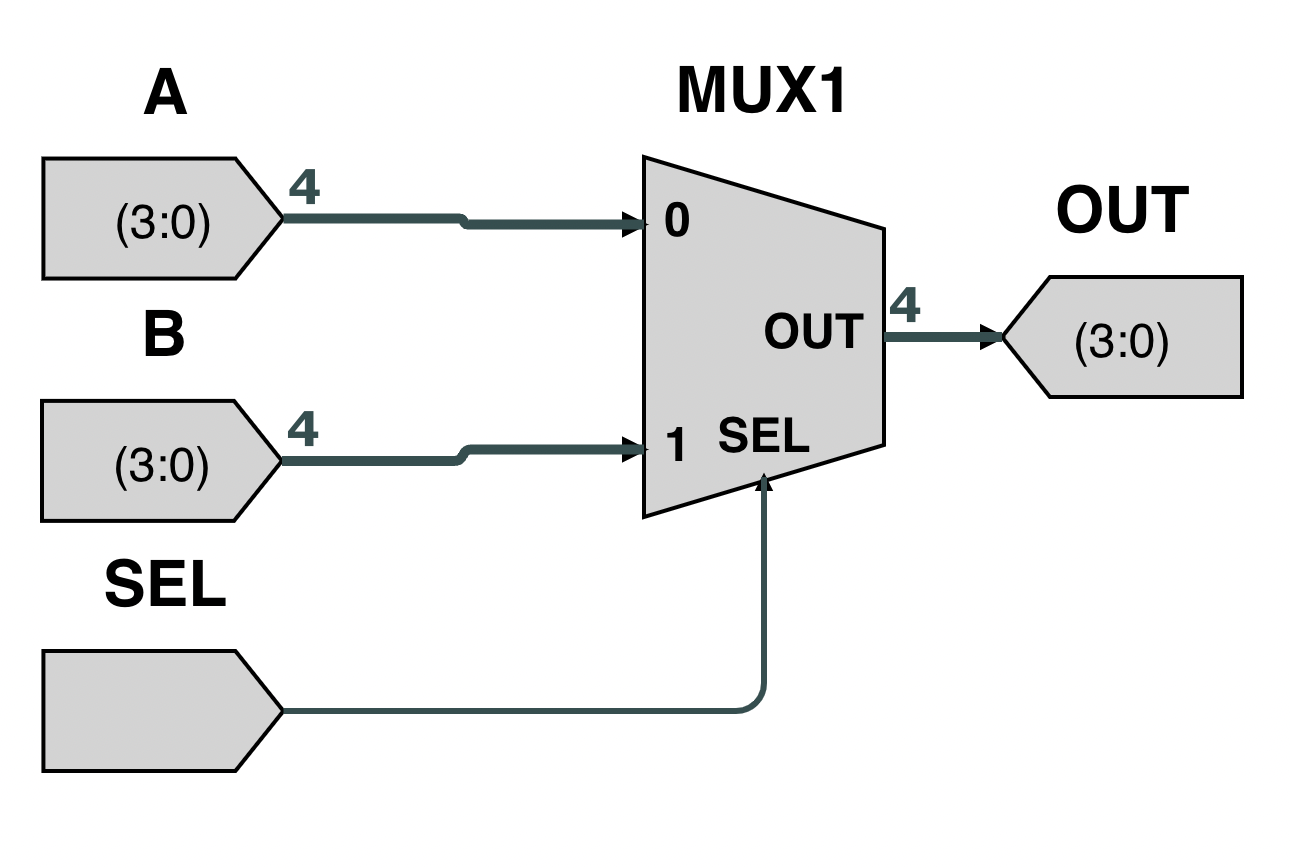
\includegraphics[width=4cm]{06.TestRes/m2.png}& \textbf{Mystery 2: Multiplexer} The second mystery sheet features a single MUX2 component which takes multi-bit inputs. This circuit was chosen as it exposes the user to truth tables which contain numbers other than 0 and 1. It also lets them DC Reduce the truth table, making it clear that B does not matter when SEL is 0, and A does not matter when SEL is 1. & 100\% \\
         \hline
         
         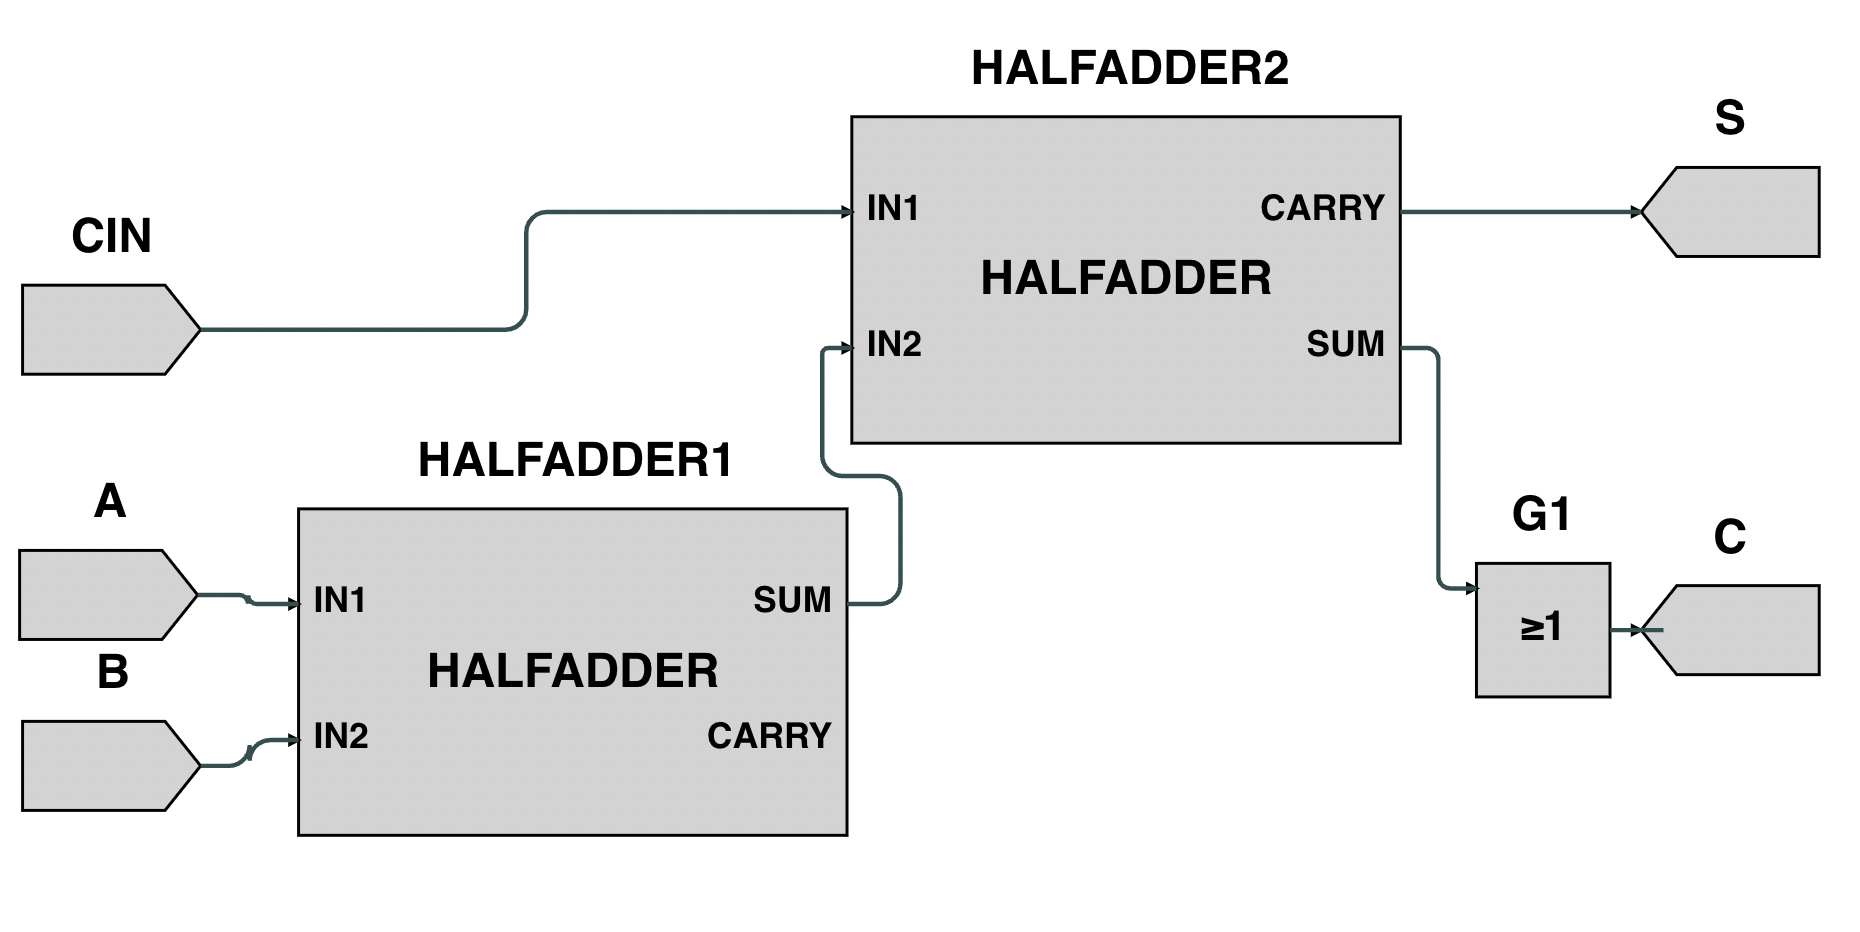
\includegraphics[width=4cm]{06.TestRes/m3.png}& \textbf{Mystery 3: Full Adder} The third mystery sheet is a full adder, which uses half adders custom components. Users can generate a truth table for the half adder alone by selecting it. This schematic also allows the user to explore algebraic reduction, as the arithmetic relationship can be inferred from the truth table. & 100\% \\
         \hline
         
         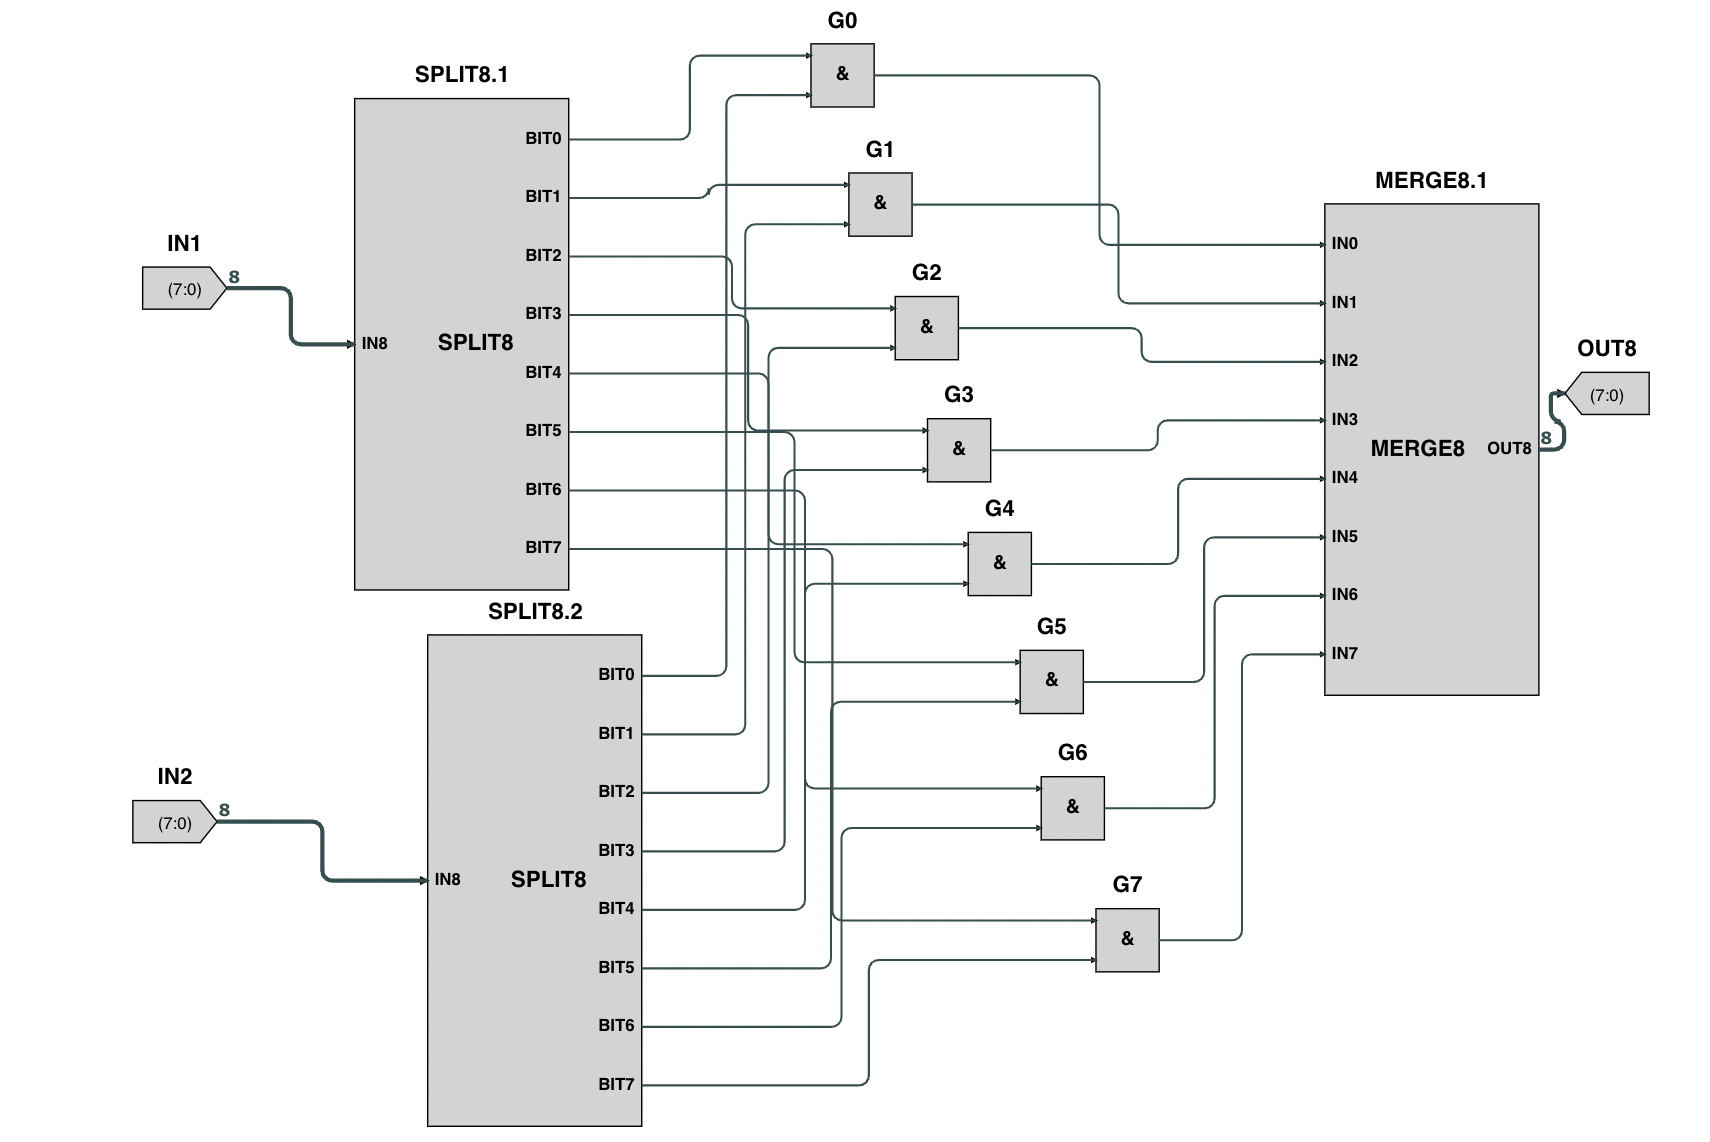
\includegraphics[width=4cm]{06.TestRes/m4.png}& \textbf{Mystery 4: Bitwise And} The fourth mystery sheet contains a large schematic with custom components and multiple wires. Such a schematic can be difficult to understand simply by looking at it. In contrast, algebraic reduction in the truth table identifies the schematic as being a simple bitwise And betwen the two inputs. & 100\% \\
         \hline
         
          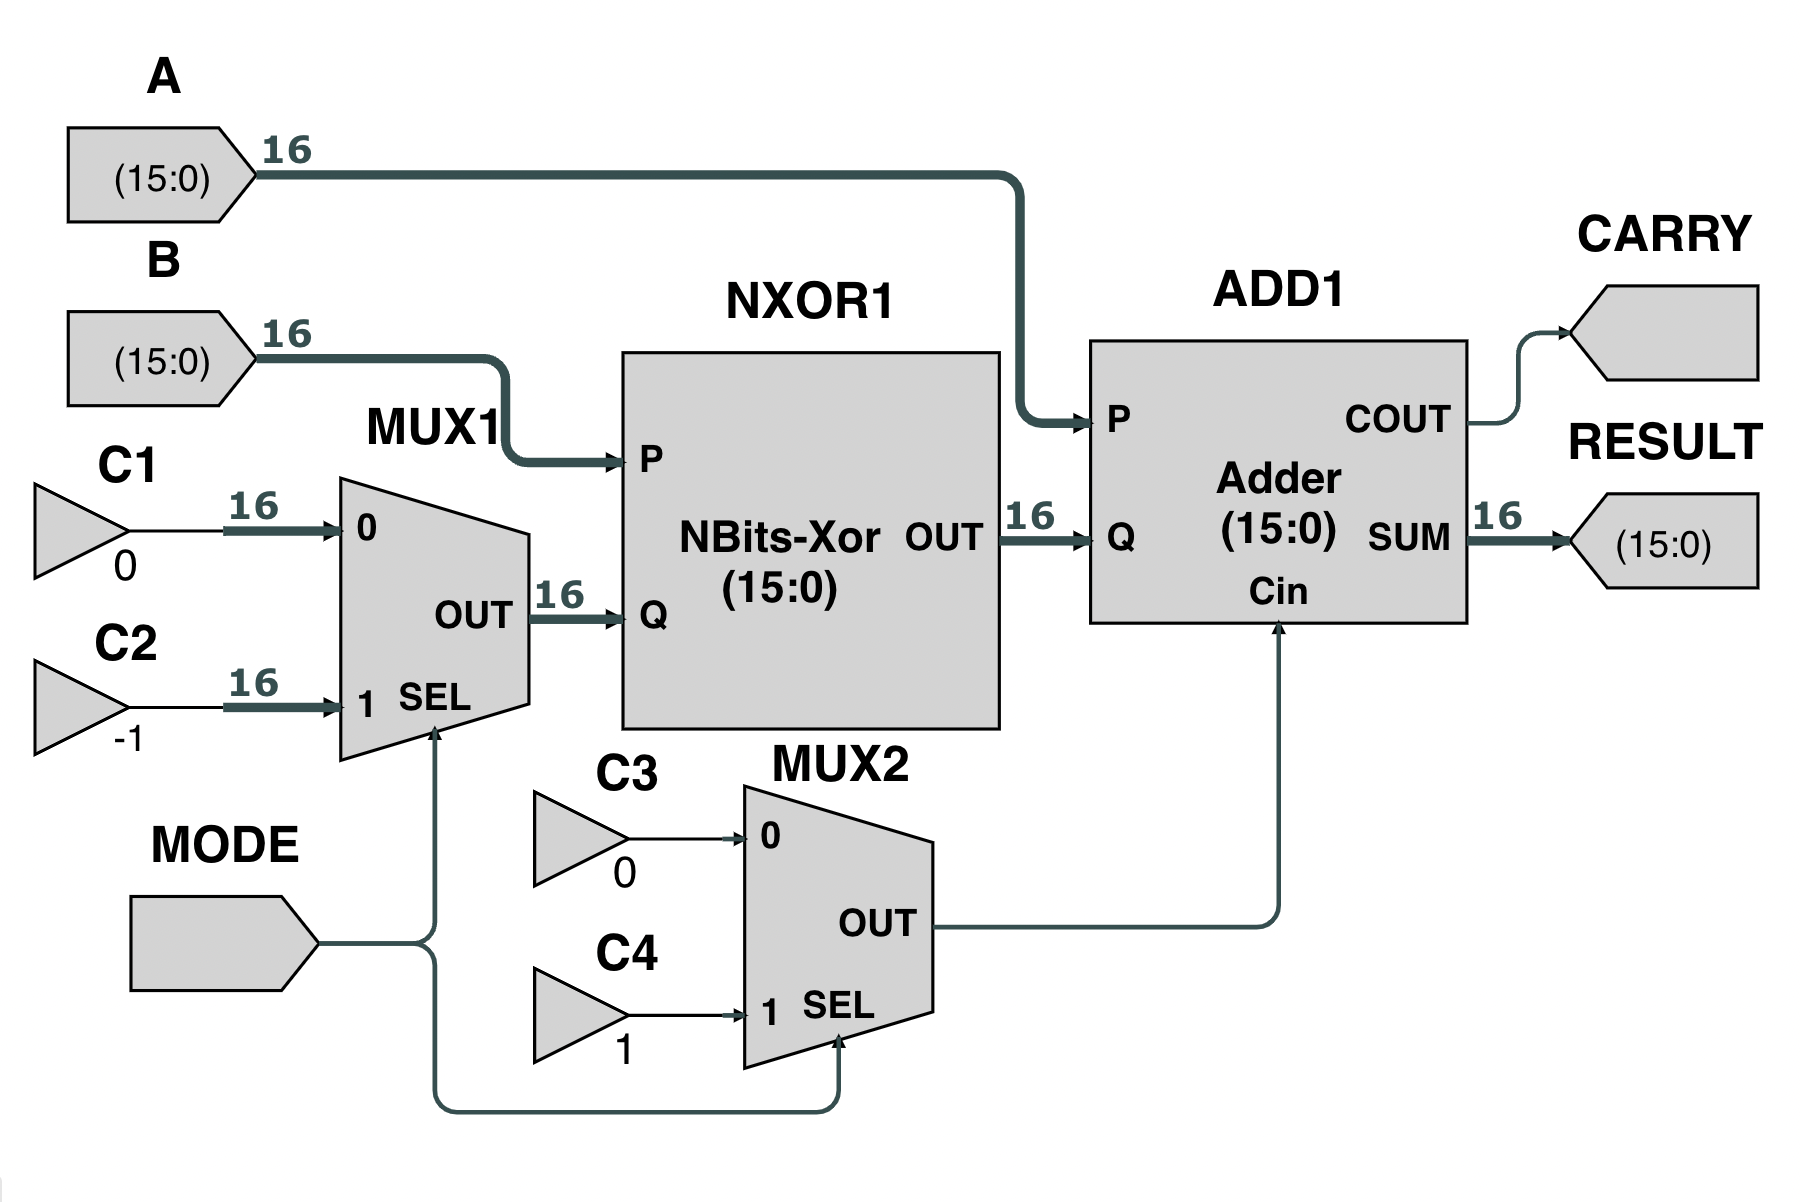
\includegraphics[width=4cm]{06.TestRes/m5.png}& \textbf{Mystery 5: Addition or Subtraction} The fifth mystery sheet incorporates Issie's built-in arithmetic components; the N-bit Adder and the N-bit XOR. The MODE input controls whether the circuit adds the two inputs, or subtracts one from the other. This circuit is more complex than the previous mystery circuits, and the inputs A and B are both 16 bits wide. This introduces the user to truth table truncation. However, using algebra, the function of the circuit can be discovered. & 90.1\% \\
         \hline
    \end{tabular}
    \caption{Mystery Sheets}
    \label{tab:mystery}
\end{table}

\begin{table}[t]
    \centering
    \begin{tabular}{|m{5cm}|m{5.5cm}|c|}
    \hline
        \textbf{Statement} & \textbf{Rationale} & \textbf{Average Score} \\ \hline
        Finding the Truth Table tab in Issie's top-level UI was easy & Evaluates the top-level UI redesign of the application. If the user can find the truth table tab easily, this means that they will likely be able to find all simulation activities. & 4.45 \\ \hline
        The functionality related to Truth Tables is clear and obvious in the UI. & Obviousness is a core principle of Issie, so evaluating whether the added features are presented in a way such that they are easy to find and understand. & 4.63 \\ 
        \hline
        Once I found a feature, it was easy to figure out what it did and how to use it. & Intuitiveness is a core principle of Issie, and this question aims to evaluate how easily the user can intuitively understand what features do. & 4.45 \\ \hline
        Using truth tables made it easier to understand the relationship between inputs and outputs in combinational logic compared to looking at the schematic. & Evaluates the effectiveness of the truth table feature set as a whole in improving the visualisation of combinational logic in Issie. & 4.36 \\ \hline
        The algebraic expressions in the truth table make it easy to understand the intended function of the circuit. & Evaluates the effectiveness of the algebraic expressions in particular for clearly communicating what the circuit does. & 4.54 \\ \hline
    \end{tabular}
    \caption{First set of questions asked in questionnaire}
    \label{tab:strongqs}
\end{table}

\begin{figure}[b]
    \centering
    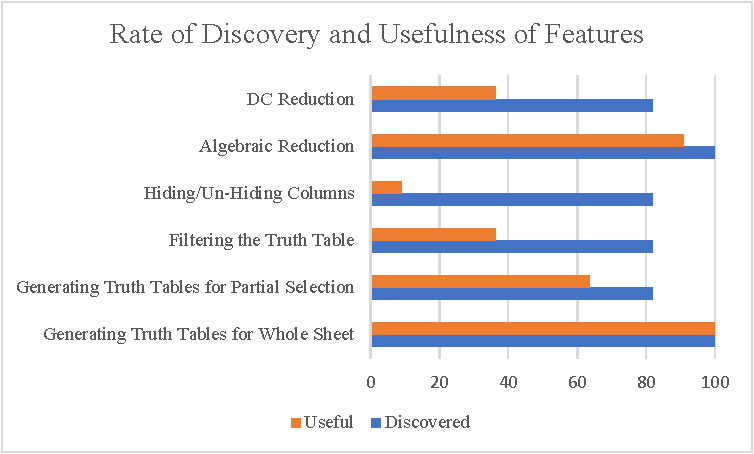
\includegraphics[width=\textwidth]{06.TestRes/graph.pdf}
    \caption{Graph showing the percentage of participants which discovered each feature and found it useful}
    \label{fig:discgraph}
\end{figure}


\section{Testing on the 8-bit ALU} \label{sec:alu}
To evaluate both the usefulness and correctness of the new combinational logic visualisation methods added to Issie, an 8- bit ALU was was analysed using the added features.
The schematic diagram of this ALU can be found in Figure \ref{fig:alu8bit} in Appendix \ref{app:alu}. The inputs into the schematic have a total width of 23 bits, yielding a theoretical truth table size of over 8 million rows. The truth table is generated in under 1 second, but truncated to 1024 rows. Due to its size, and given that the exact specification of the ALU was not known at that point, the numeric truth table was not massively useful. However, had the specification been known prior to analysis, the numeric truth table would have undoubtedly been useful for checking the correctness of multiple input/output combinations. In order to further understand the ALU functions, algebraic reduction was used. The inputs $A$, $B$, and $CIN$ were set as algebra; this reduced the truth table size from over 8 million rows to 64. The first 18 rows of this algebraic truth table can be seen in Figure \ref{fig:alutable}. The other inputs, $X$ and $F$, eventually propagate to the SEL ports of multiplexers and therefore cannot be set as algebra. However, this works out very well -- these inputs control the behaviour of the ALU, meaning that it is better for their values to stay as numbers in the truth table. For each combination of these control inputs, a different expression at the output of the ALU ($OUT$) can be observed. From the algebraic truth table, the logical function of the ALU was described using eight short statements:
\begin{enumerate}
    \item When $X = 0$ and $F = 0$, $OUT$ is the sum of A and B
    \item When $X = 0$ and $F = 2$, $OUT = A - B$
    \item When $X = 0$ and $F = 6$, $OUT = CIN + A - B$
    \item When $X = 0$ and $F = 4$, $OUT$ is the sum of A, B, and CIN
    \item When $X = 0$ and $F[0] = 1$ (i.e. F is odd), $OUT = B$
    \item When $X = 1$, $OUT = A \& B$
    \item When $X = 2$ or $X = 3$, $OUT$ is the XOR of A and B
    \item Otherwise, $OUT$ is $B$ right-shifted by 1.
\end{enumerate}

\begin{figure}
    \centering
    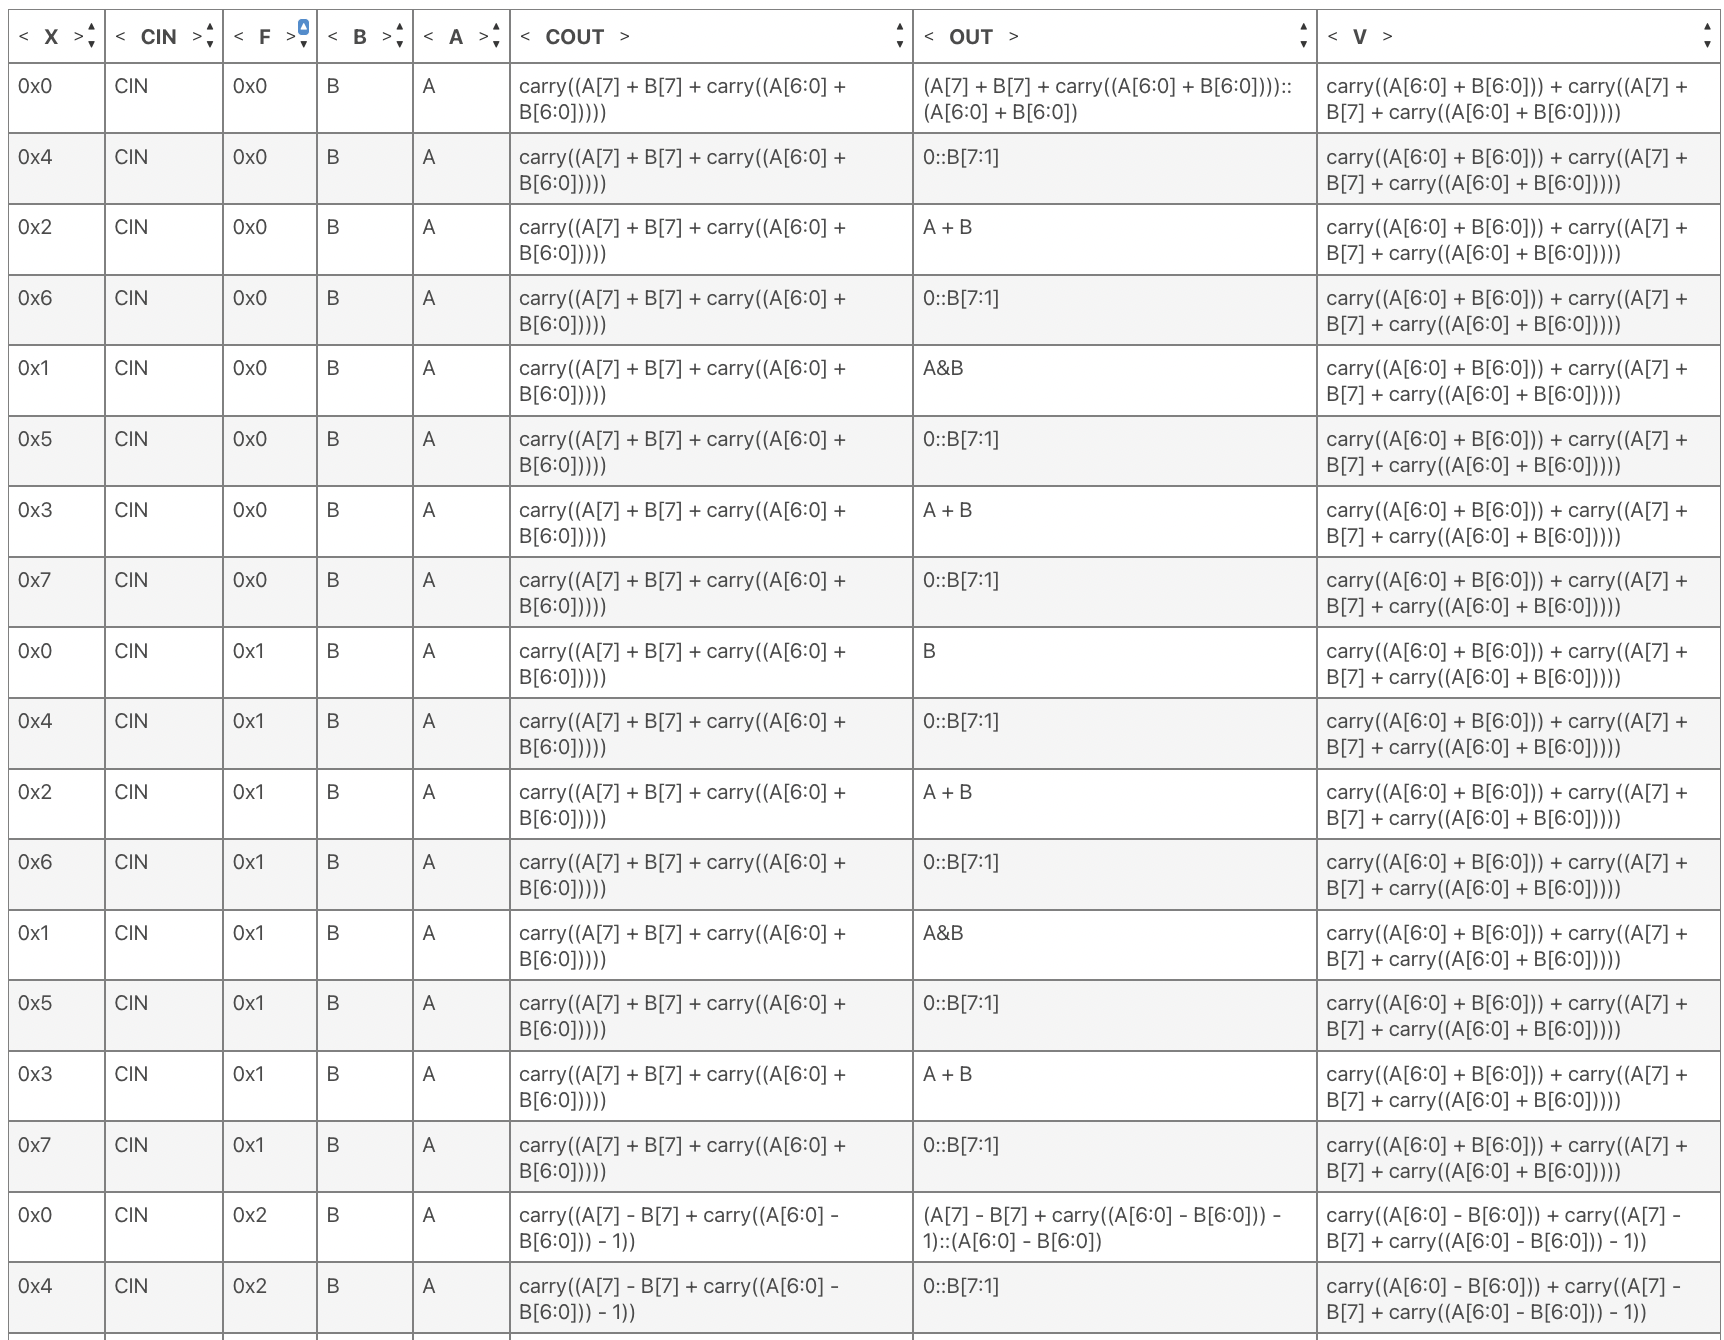
\includegraphics[width=\textwidth]{06.TestRes/alutable.png}
    \caption{First 18 rows of the Algebraic Truth Table for 8-bit ALU}
    \label{fig:alutable}
\end{figure}